% Choose one to switch between slides and handout
%\documentclass[]{beamer}
\documentclass[handout]{beamer}

% Video Meta Data
\title{Bitcoin, Blockchain and Cryptoassets}
\subtitle{Payment Systems}
\author{Prof. Dr. Fabian Schär}
\institute{University of Basel}

% Config File
% Packages
\usepackage[utf8]{inputenc}
\usepackage{hyperref}
\usepackage{gitinfo2}
\usepackage{tikz}
\usepackage{amsmath}
\usepackage{bibentry}
\usepackage{xcolor}
\usepackage{colortbl} % Add colour to LaTeX tables
\usepackage{caption}
\usepackage[export]{adjustbox}
\usepackage{pgfplots} \pgfplotsset{compat = 1.17}

% Color Options
\definecolor{highlight}{rgb}{0.65,0.84,0.82}
\definecolor{focus}{rgb}{0.72, 0, 0}

% Beamer Template Options
\beamertemplatenavigationsymbolsempty
\setbeamertemplate{footline}[frame number]
\setbeamercolor{structure}{fg=black}
\setbeamercolor{footline}{fg=black}
\setbeamercolor{title}{fg=black}
\setbeamercolor{frametitle}{fg=black}
\setbeamercolor{item}{fg=black}
\setbeamercolor{}{fg=black}
\setbeamercolor{bibliography item}{fg=black}
\setbeamercolor*{bibliography entry title}{fg=black}
\setbeamertemplate{items}[square]
\setbeamertemplate{enumerate items}[default]
\captionsetup[figure]{labelfont={color=black},font={color=black}}
\captionsetup[table]{labelfont={color=black},font={color=black}}

\setbeamertemplate{bibliography item}{\insertbiblabel}

% Link Icon Command
\newcommand{\link}{%
    \tikz[x=1.2ex, y=1.2ex, baseline=-0.05ex]{%
        \begin{scope}[x=1ex, y=1ex]
            \clip (-0.1,-0.1)
                --++ (-0, 1.2)
                --++ (0.6, 0)
                --++ (0, -0.6)
                --++ (0.6, 0)
                --++ (0, -1);
            \path[draw,
                line width = 0.5,
                rounded corners=0.5]
                (0,0) rectangle (1,1);
        \end{scope}
        \path[draw, line width = 0.5] (0.5, 0.5)
            -- (1, 1);
        \path[draw, line width = 0.5] (0.6, 1)
            -- (1, 1) -- (1, 0.6);
        }
    }

% Read Git Data from Github Actions Workflow
% Defaults to gitinfo2 for local builds
\IfFileExists{gitInfo.txt}
	{\input{gitInfo.txt}}
	{
		\newcommand{\gitRelease}{(Local Release)}
		\newcommand{\gitSHA}{\gitHash}
		\newcommand{\gitDate}{\gitAuthorIsoDate}
	}

% Custom Titlepage
\defbeamertemplate*{title page}{customized}[1][]
{
  \vspace{-0cm}\hfill
\includegraphics[width=2.5cm]{../config/logo_cif}
  
\includegraphics[width=1.9cm]{../config/seal_wwz}
  \\ \vspace{2em}
  \usebeamerfont{title}\textbf{\inserttitle}\par
  \usebeamerfont{title}\usebeamercolor[fg]{title}\insertsubtitle\par  \vspace{1.5em}
  \small\usebeamerfont{author}\insertauthor\par
  \usebeamerfont{author}\insertinstitute\par \vspace{2em}
  \usebeamercolor[fg]{titlegraphic}\inserttitlegraphic
    \tiny \noindent \texttt{Release Ver.: \gitRelease}\\ 
    \texttt{Version Hash: \gitSHA}\\
    \texttt{Version Date: \gitDate}\\ \vspace{1em}
  \link \href{https://github.com/cifunibas/Bitcoin-Blockchain-Cryptoassets/blob/main/slides/intro.pdf}
  {Get most recent version}\\
  \link \href{https://github.com/cifunibas/Bitcoin-Blockchain-Cryptoassets/blob/main/slides/intro.pdf}
  {Watch video lecture}\\ \vspace{1em}
  License: \texttt{Creative Commons Attribution-NonCommercial-ShareAlike 4.0 International}\\\vspace{2em}
  
\includegraphics[width = 1.2cm]{../config/license}
}

% tikzlibraries
\usetikzlibrary{decorations.pathreplacing}
\usetikzlibrary{decorations.markings}
\usetikzlibrary{positioning}

%caption font
\captionsetup{font=footnotesize}


%%%%%%%%%%%%%%%%%%%%%%%%%%%%%%%%%%%%%%%%%%%%%%
%%%%%%%%%%%%%%%%%%%%%%%%%%%%%%%%%%%%%%%%%%%%%%
\begin{document}

\thispagestyle{empty}
\begin{frame}[noframenumbering]
	\titlepage
\end{frame}

%%%
\begin{frame}{Payment Systems: Today's Challenge}

Physical Cash: Presence in the same place at the same time
\begin{figure}[h]
	\center
		    
\begin{tikzpicture}[scale = 0.67]

% Payee
	\node 			(payee) at (12,0) {
\includegraphics[height = 1.6cm]{../assets/images/agents/reaching_left.png}};

% Payer
	\node 			(payer) at (0,0) {
\includegraphics[height = 1.6cm]{../assets/images/agents/handing_right.png}};
	

% Goods vs. Money flow
	
	\draw[->, thick, dashed]	([yshift=1cm]payer.south east) -- ([yshift=1cm]payee.south west) node[midway, fill=white] {Cash};

	\draw[<-, thick]		([yshift=-1cm]payer.north east) -- ([yshift=-1cm]payee.north west) node[midway, fill=white] {Goods / Services};

	
\end{tikzpicture}

\end{figure}

\vspace{1.5 em}

\uncover<2->{Digital Cash: Proof of ownership
\begin{figure}[h]
	\center
		    
\begin{tikzpicture}[scale = 0.67]

% Payee
\node 			(payee) at (12,0) {
\includegraphics[width = 1.2 cm]{../assets/images/avatar.png}};


% Payer
\node 			(payer) at (0,0) {
\includegraphics[width = 1.2 cm]{../assets/images/avatar.png}};


% Goods vs. Money flow	
	\draw[->, thick, dashed]	([yshift=0.5cm]payer.south east) -- ([yshift=0.5cm]payee.south west) 
						node[midway, fill=white] {Digital Cash};

	\draw[<-, thick]	([yshift=-0.5cm]payer.north east) -- ([yshift=-0.5cm]payee.north west) node[midway, fill=white] {Goods / Services};


% Copy-Paste Symbol
	
	\coordinate	(A) at ([xshift=-0.1cm, yshift=-0.1cm]payer.south west);
	\coordinate	(B) at ([xshift = 1.2cm, yshift = -0.8cm]A);
	\coordinate	(C) at ([xshift = 1.6cm]A);
	\coordinate	(D) at ([xshift = 1.3cm]B);
	\coordinate (E) at ([xshift = 1.5cm, yshift = -0.4cm]A);
	
	\draw[rounded corners=5pt, focus, very thick]	(A) rectangle (B) node [midway, focus] {Ctrl};
	\draw[rounded corners=5pt, focus, very thick]	(C) rectangle (D) node [midway, focus] {\scriptsize{C/V}};
	
	%\draw (E) node [midway, focus] {+};
	


	 
\end{tikzpicture}

\end{figure}}
	
\end{frame}
%%%	

%%%
\begin{frame}{Today's Solution: Intermediaries Keeping Money Registries}

\begin{figure}[h]
	\center
		    
\begin{tikzpicture}[scale = 0.67]

% Payee
\node 			(payee) at (12,0) {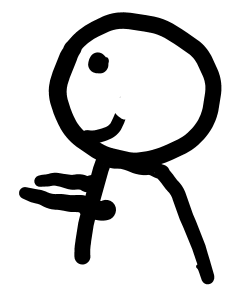
\includegraphics[height = 1.6cm]{../assets/images/avatar_left.png}};


% Payer
\node 			(payer) at (0,0) {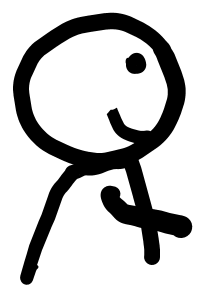
\includegraphics[height = 1.6cm]{../assets/images/avatar_right.png}};


% Intermediary
\node 			(intermediary) at (6,-2.5) {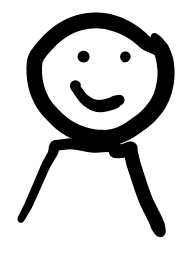
\includegraphics[height = 1.6cm]{../assets/images/avatar_rand3.png}};


% Goods vs. Money flow	
	\draw[->, thick, dashed]	([yshift=1cm] payer.south east) -- (intermediary.west) 
						node[midway, fill=white] {Payment order};
						
\draw[->, thick, dashed]	(intermediary.east) -- ([yshift=1cm] payee.south west) 
						node[midway, fill=white] {Credit note};

	\draw[<-, thick]	(payer.east) -- (payee.west) node[midway, fill=white] {Goods / Services};


% Registry

\coordinate	(A) at (0.8,-2.5);
\coordinate	(B) at (2.4,-2.5);
\coordinate	(C) at (4,-2.5);
\coordinate	(D) at (8,-2.5);
\coordinate	(E) at (9.6,-2.5);
\coordinate	(F) at (11.2,-2.5);
\coordinate	(G) at (2.4,-4.5);
\coordinate	(H) at (9.6,-4.5);

\draw[thick,focus]	(A) -- (C);
\draw[thick,focus]	(B) -- (G);
\draw[thick,focus]	(D) -- (F);
\draw[thick,focus]	(E) -- (H);

\node[draw=none, fill=none]	at(0.7,-2.8)[focus,right]{\tiny Amount};
\node[draw=none, fill=none]	at(11.3,-2.8)[focus,left]{\tiny Amount};


	


	 
\end{tikzpicture}

\end{figure}

\uncover<2->{\vspace{1 em}

\textbf{Registry Types}\\
\vspace{1 em}
\textbf{Implicit:} Verbal agreements, limited to small groups.\\
\textbf{Explicit:} Records in written or digital databases.}
	
\end{frame}
%%%	

%%%
\begin{frame}{Implicit Registry Example: The Stone Money of Yap}
	\center
	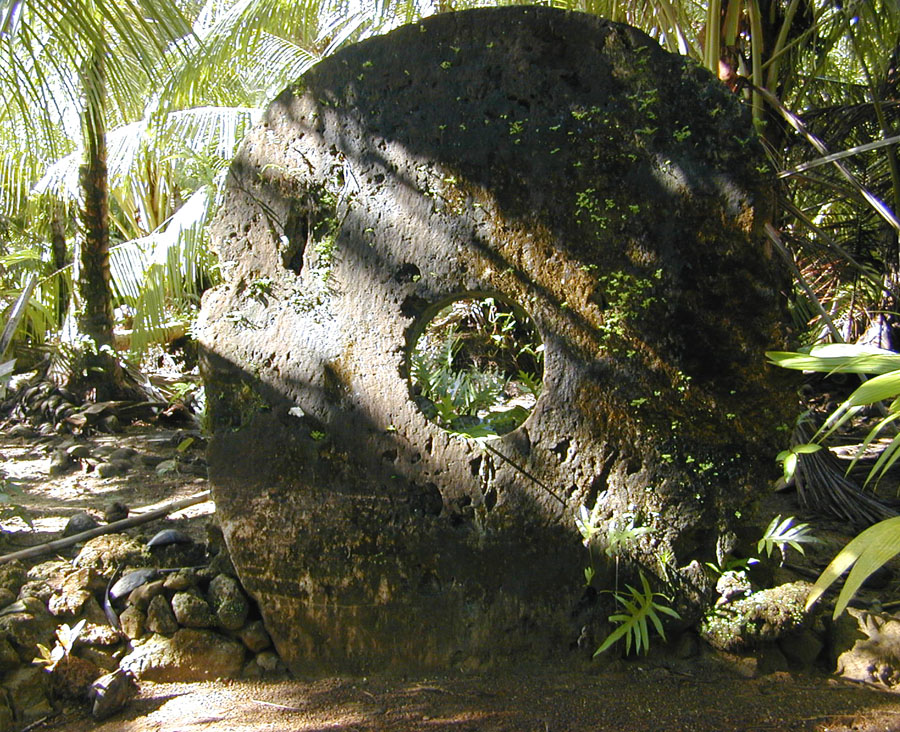
\includegraphics[width=8cm]{../assets/images/yap_stones}\\
	\footnotesize{Picture source: Eric Guinther}
\end{frame}


%%%
\begin{frame}{Implicit Registry Example: The Stone Money of Yap}

\begin{figure}[h]
	\center
		


\begin{tikzpicture}[scale = 0.67]

\definecolor {dgray}{rgb}{122,122,122}
\definecolor {lgray}{rgb}{194,194,194}

% Payee
	\node 			(payee) at (12,7) {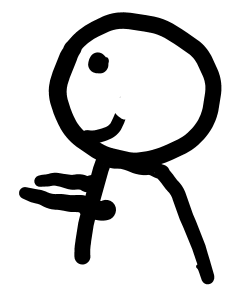
\includegraphics[height = 1.6cm]{../assets/images/avatar_left.png}};

% Payer
	\node 			(payer) at (0,7) {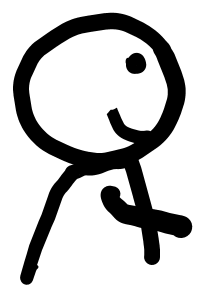
\includegraphics[height = 1.6cm]{../assets/images/avatar_right.png}};
	

% Stone
	\node (outer) at (10.5,1.5) [circle, minimum width=2.5cm, draw = gray, fill = lightgray]{};

	\node (inner) at (10.5,1.5) [circle, minimum width=0.9cm, draw = gray, fill = white]{};


% Network
	\node			(agenta) at (1,2.8) {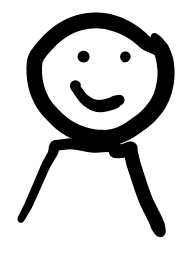
\includegraphics[width = 0.6 cm]{../assets/images/avatar_rand3.png}};
	\node 			(agentb) at (0.5,1) {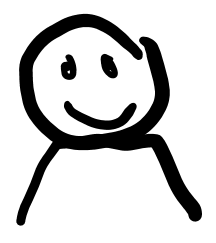
\includegraphics[width = 0.6 cm]{../assets/images/avatar_rand4.png}};
	\node 			(agentc) at (3,2.1) {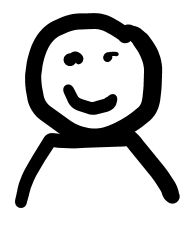
\includegraphics[width = 0.6 cm]{../assets/images/avatar_rand5.png}};
	\node 			(agentd) at (2.8,0) {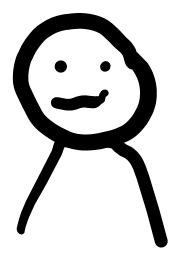
\includegraphics[width = 0.6 cm]{../assets/images/avatar_rand1.png}};
	\node 			(agente) at (5,4.3) {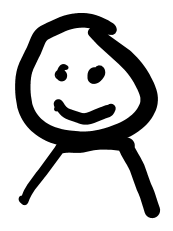
\includegraphics[width = 0.6 cm]{../assets/images/avatar_rand2.png}};	
	\node 			(agentf) at (5.1,1.1) {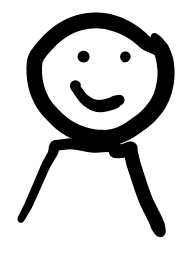
\includegraphics[width = 0.6 cm]{../assets/images/avatar_rand3.png}};
	\node 			(agentg) at (7.5,3.8) {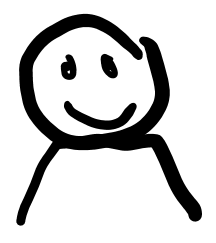
\includegraphics[width = 0.6 cm]{../assets/images/avatar_rand4.png}};
	\node 			(agenth) at (6.7,0.4) {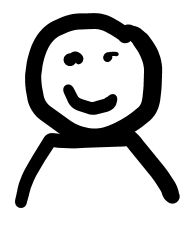
\includegraphics[width = 0.6 cm]{../assets/images/avatar_rand5.png}};	
	

% Goods vs. Money flow
	
	\draw[->, thick, dashed]	([yshift=1cm]payer.south east) -- ([yshift=1cm]payee.south west) node[midway, fill=white] {Stone Property Rights};
	
	\draw[->, thick, dashed]	(payer.south) -- (agenta.north) node[midway, fill=white, align = center, text = focus] {\footnotesize "Payee is new owner\\ \footnotesize of stone XY"};

	\draw[<-, thick]		([yshift=-1cm]payer.north east) -- ([yshift=-1cm]payee.north west) node[midway, fill=white] {Goods / Services};
	
% Network flow


	\draw[<->, thick, dashed]	(agenta.south) -- (agentb.north);
	\draw[<->, thick, dashed] 	(agenta.east) -- (agente.west);
	\draw[<->, thick, dashed]	(agenta.south east) -- (agentc.west);
	\draw[<->, thick, dashed]	(agente.south west) -- (agentc.north east);
	\draw[<->, thick, dashed]	(agente.south) -- (agentf.north);
	\draw[<->, thick, dashed]	(agente.east) -- (agentg.west);
	\draw[<->, thick, dashed]	(agentc.south west) -- (agentb.east);
	\draw[<->, thick, dashed]	(agentc.south) -- (agentd.north);
	\draw[<->, thick, dashed]	(agentc.south east) --  (agentf.west);
	\draw[<->, thick, dashed]	(agentg.south west) -- (agentf.north east);
	\draw[<->, thick, dashed]	(agentg.south) -- (agenth.north);
	\draw[<->, thick, dashed]	(agentb.south east) -- (agentd.west);
	\draw[<->, thick, dashed]	(agentf.south west) -- (agentd.east);
	\draw[<->, thick, dashed]	(agentf.south east) -- (agenth.west);
	\draw[<->, thick, dashed]	(agenth.south west) -- (agentd.east);
	
\end{tikzpicture}

\end{figure}
	
\end{frame}
%%%

%%%
\begin{frame}{Closed Loop Payment Systems}

\textbf{Defining Characteristics}
 	\begin{itemize}
 		\item Direct relationships with both, payer and payee.
 		\item One operator, one set of rules.
 	\end{itemize}
\vspace{1.5em}

\uncover<2->{\textbf{Examples of Closed Loop Systems}
 	\begin{itemize}
 		\item Merchant issued payment cards
 		\item Western Union
 		\item PayPal
 		\item Several mobile payment services: MPesa, WeChat		
 	\end{itemize}}
\vspace{1.5em}

\uncover<3->{
$\Rightarrow$ Highly efficient but utility depends on number of end-users.
}
	
\end{frame}
%%%	

%%%
\begin{frame}{Open Loop Payment Systems}

\begin{figure}[h]
	\center
		    
\begin{tikzpicture}[scale = 0.67]

% Flow




% Payee
	\node 			(payee) at (11.25,-1.51) {
\includegraphics[width = 1 cm]{../assets/images/avatar.png}};

% Payer
	\node 			(payer) at (-1.75,-1.51) {
\includegraphics[width = 1 cm]{../assets/images/avatar.png}};
	

% Payment networks & Flow



	\draw [line width=4,lightgray]  		(0,0) -- (3.5,0);
	\draw [line width=4,lightgray]  		(0.875,1.51) -- (2.625,-1.51);
	\draw [line width=4,lightgray]  		(2.625,1.51) -- (0.875,-1.51);
	\draw [draw = focus, thick, fill=lightgray]	(0,0) circle (0.7);
	\draw [draw = white, fill=lightgray]	(3.5,0) circle (0.7);
	\draw [draw = white, fill=lightgray]	(0.875,1.51) circle (0.7);
	\draw [draw = focus, thick, fill=lightgray]	(2.625,1.51) circle (0.7);
	\draw [draw = white, fill=lightgray]	(0.875,-1.51) circle (0.7);
	\draw [draw = white, fill=lightgray]	(2.625,-1.51) circle (0.7);

	\draw [line width=4,lightgray]  		(6,0) -- (9.5,0);
	\draw [line width=4,lightgray]  		(6.875,1.51) -- (8.625,-1.51);
	\draw [line width=4,lightgray]  		(8.625,1.51) -- (6.875,-1.51);
	\draw [draw = white, fill=lightgray]	(6,0) circle (0.7);
	\draw [draw = white, fill=lightgray]	(9.5,0) circle (0.7);
	\draw [draw = focus, thick, fill=lightgray]	(6.875,1.51) circle (0.7);
	\draw [draw = focus, thick, fill=lightgray]	(8.625,1.51) circle (0.7);
	\draw [draw = white, fill=lightgray]	(6.875,-1.51) circle (0.7);
	\draw [draw = white, fill=lightgray]	(8.625,-1.51) circle (0.7);

	
	
	\draw [draw = focus, fill=lightgray]	(11.25,1.51) circle (0.7); % Correspondent Bank



% Border and Labels

	\draw [line width=1.5,gray] 	(4.75,2.5) -- (4.75, -2.5) node [below, black] {\footnotesize Border};
 
	\draw 	(1.75,-2.5) node [below, black] {\footnotesize Network A};
	
	\draw 	(7.75,-2.5) node [below, black] {\footnotesize Network B};
	
	\draw 	(-1.75,-2.5) node [below, black] {\footnotesize Payer};
	
	\draw 	(11.25,-2.5) node [below, black] {\footnotesize Payee};

% Flow and clearing houses

	\draw[->, dashed, line width = 1.5, focus]	(payer.north) -- (-1.75,0) -- (-0.7,0);
	
	\draw[line width = 1.5, focus]	(0.7,0) -- (1.75,0) -- (2.2725,0.91);
	
	\draw[<->, dashed, line width = 1.5, focus]	(3.325,1.51) -- (6.175,1.51);
	
	\draw[line width = 1.5, focus]	(7.225,0.91) -- (7.75,0) -- (8.2725,0.91);
	
	\draw[<->, dashed, line width = 1.5, focus]	(9.325,1.51) -- (10.55,1.51);
	
	\draw[->, dashed, line width = 1.5, focus]	(11.25,0.81) -- (payee.north);
	
	\node (CH1) at (1.75,0) {
\includegraphics[width = 0.8 cm]{../assets/images/bank.png}};
		
	\node (CH2) at (7.75,0) {
\includegraphics[width = 0.8 cm]{../assets/images/bank.png}};


	
\end{tikzpicture}

\end{figure}
\vspace{1em}

\uncover<2->{\textbf{Multiple relationships and rule sets lead to compounding of:}
 	\begin{itemize}
 		\item Processing time (from switch to settlement)
 		\item Fees (subscription and transaction based)
 		\item Network dependencies
 		\item Exception handling cost (fraud, errors, underfunding)		
 	\end{itemize}}

	
\end{frame}
%%%	

%%%
\begin{frame}{Network Examples}

\textbf{SWIFT}, global scope, since 1970s\\
Standardized transaction \textit{messaging }system.

\vspace{1em}

\textbf{SEPA}, EU and EFTA, since 2008/2009\\
Payment network for low cost EUR payments with a maximum transmission time.

\vspace{1em}

\textbf{Credit Card Networks}, e.g. Visa, Mastercard\\
Focus on consumer transactions in multiple currencies. 

\vspace{1em}

\textbf{National Payment Networks}, e.g., SIC, CHIPS, FedWire.\\ 
Connecting parties in one currency and one regulatory environment.

\end{frame}
%%%	

%%%
\begin{frame}{Bitcoin as a Solution?}

\begin{itemize}
	\item A physical cash payment system does not meet today's needs.
	\item<2-> Today's digital payment solutions depend on one or several centrally maintained registries and proprietary networks.
	\item<3-> Centralized registries and proprietary networks introduce single points of failure or attacks, i.e., the risk of data loss, manipulation, or censorship.
\end{itemize}
\vspace{1em}

\uncover<4->{
$\Rightarrow$ A desirable solution would \color{focus} combine the efficiency of digitalization without dependency on centralized registries \color{black} and intermediaries. 
}	
\end{frame}
%%%	

%%%
\begin{frame}%[allowframebreaks]
\frametitle{References and Recommended Reading}

		\begin{columns}[T]
			\begin{column}{0.1\textwidth}
					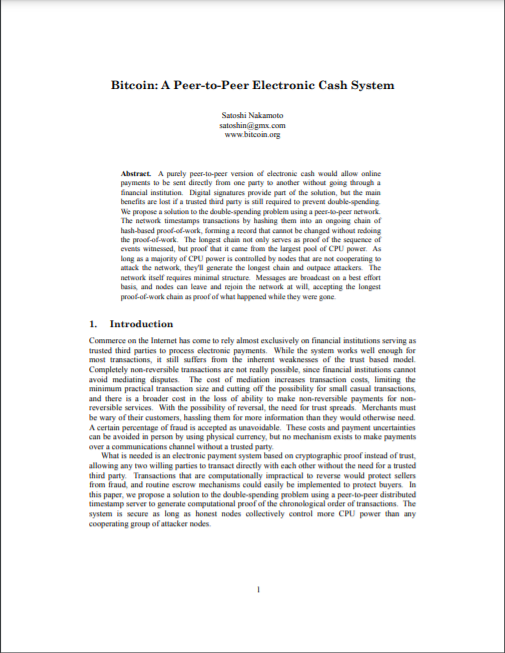
\includegraphics[width = 1.7cm, frame]{../assets/images/nakamoto_cover}
			\end{column} %\hfill
			\begin{column}{0.8\textwidth}
				\textbf{Bitcoin: A Peer-to-Peer Electronic Cash System} \\ 
				Satoshi Nakamoto \\
				\link \href{https://bitcoin.org/bitcoin.pdf}{Online version}
			\end{column}
		\end{columns}
	%
	\vspace{1.5em}
	%
	\uncover<2->{
		\begin{columns}[T]
			\begin{column}{0.1\textwidth}
					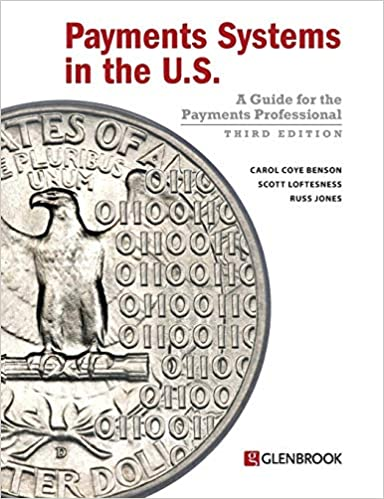
\includegraphics[width = 1.7cm, frame]{../assets/images/benson_cover}
			\end{column} %\hfill
			\begin{column}{0.8\textwidth}
				\textbf{Payments Systems in the U.S.} \\ 
				Carol Coye Benson \\
				\texttt{ISBN: 978-0982789742}
			\end{column}
		\end{columns}
	}
	%
	\vspace{1.5em}
	%
	

\end{frame}
%%%


\end{document}
